\documentclass[conference]{IEEEtran}

\usepackage[spanish]{babel}
\usepackage{amsmath,amssymb,amsfonts,amsthm}
\usepackage{graphicx}
\usepackage[utf8]{inputenc} % Caracteres en Español (Acentos, ñs)
\usepackage{url} % ACENTOS
\usepackage{hyperref} % Referencias
\usepackage{subfig}
\usepackage{lipsum}
\usepackage{balance} 
\usepackage{etoolbox}
\makeatletter
\patchcmd{\frontmatter@RRAP@format}{(}{}{}{}
\patchcmd{\frontmatter@RRAP@format}{)}{}{}{}
\makeatother	

\usepackage[backend=bibtex,sorting=none]{biblatex}
\setcounter{biburllcpenalty}{7000}
\setcounter{biburlucpenalty}{8000}
\addbibresource{references.bib}

% fecha
\usepackage{datetime}
\newdateformat{specialdate}{
    \twodigit{\THEDAY}-\twodigit{\THEMONTH}-\THEYEAR
}
\date{\specialdate\today}

% la sentencia \burl en las citas... 
\usepackage[hyphenbreaks]{breakurl}
\renewcommand\spanishtablename{Tabla}
\renewcommand\spanishfigurename{Figura}


\begin{document}
% Definitions
\newcommand{\breite}{0.9} %  for twocolumn
\newcommand{\RelacionFiguradoscolumnas}{0.9}
\newcommand{\RelacionFiguradoscolumnasPuntoCinco}{0.45}

%Title of paper
\title{Reporte de Laboratorio 2 \\ Conteo de Frutos Pequeños en Tiempo Real Utilizando una Plataforma Giratoria}

% Trabajo Individual
\author{
    \IEEEauthorblockN{
        Ricardo Emmanuel Uriegas Ibarra\IEEEauthorrefmark{1}
        }
    % En caso de trabajos en equipo, poner a todos los autores 
    % en estricto ORDEN ALFABETICO
    %\author{\IEEEauthorblockN{Michael Shell\IEEEauthorrefmark{1},
    %Homer Simpson\IEEEauthorrefmark{1}}
    \IEEEauthorblockA{
        \IEEEauthorrefmark{1}Ingeniería en Tecnologías de la Información\\
        Universidad Politécnica de Victoria
    }
}

\maketitle

%%%%%%%%%%%%%%%%%%%%%%%%%%%%%%%%%%%%%%%%%%%%%%%%%%%%%%%%%%%%%%%%%%%%%%%
\begin{abstract} 
    
\end{abstract}

%%%%%%%%%%%%%%%%%%%%%%%%%%%%%%%%%%%%%%%%%%%%%%%%%%%%%%%%%%%%%%%%%%%%%%%
\section{Introducción}
La disponibilidad de metodologías prácticas y fiables de detección de frutos en campo resulta fundamental para realizar previsiones precisas de la cosecha\cite{}. 


%%%%%%%%%%%%%%%%%%%%%%%%%%%%%%%%%%%%%%%%%%%%%%%%%%%%%%%%%%%%%%%%%%%%%%%
\section{Desarrollo Experimental}
En este trabajo se presenta un sistema de detección en tiempo real de frutos pequeños que giran en una plataforma giratoria.

Para lograr esto se necesita conocimiento en las siguientes áreas:
\begin{itemize}
    \item Procesamiento de Imágenes
    \item Visión por Computadora
    \item Redes Neuronales
\end{itemize}

La mayor parte de estos conocimientos los hemos aprendido en unidades previas de la materia, por lo que no se abordarán en este reporte.

\subsection{Dataset}
Antes de todo debemos definir que es un dataset y porque es que lo ocupamos en este trabajo.
Un dataset es un conjunto de datos que se utilizan para entrenar un modelo de machine learning. En este caso, el dataset que se utilizó fue totalmente recolectado por nosotros mismos; de algunos frutos variados,\cite{} el cual consiste en imágenes de frutos chicos en diferentes entornos; esto porque se creia que el proyecto debia abarcar todo tipo de frutos. El dataset se componen de 1 sola clase, la cual es la de fruto. La cantidad de imágenes recolectada fue de 38 imágenes, pero realizando aumentacion de datos se logro llegar a 114 imágenes recolectadas por el equipo.

Las técnicas de augmentation que se aplicaron a los datos recolectados fueron los siguientes:
\begin{itemize}
    \item Flip: Horizontal, Vertical
    \item Rotación 90°: En sentido horario, antihorario, al revés
    \item Crop: 0\% mínimo, 20\% máximo
    \item Rotación: Entre -15° y +15°
    \item Shear: ±10° Horizontal, ±10° Vertical
    \item Hue: Entre -15° y +15°
    \item Saturación: Entre -25\% y +25\%
    \item Brillo: Entre -15\% y +15\%
    \item Exposición: Entre -10\% y +10\%
    \item Blur: Hasta 2.5px
    \item Ruido: Hasta 0.1\% de píxeles
\end{itemize}

\subsection{Modelo}
Debido a la baja cantidad de imágenes para entrenamiento que poseíamos, sumado a la eficiencia que debía de poseer el modelo para ser ejecutado en tiempo real, se opto por usar el modelo pre-entrenando para detección de objetos de la librería ultralytics\cite{} yolov8n\cite{}.

\subsection{Entrenamiento}
Una vez ya se tenia la selección del modelo pre-entrenado a usar, se prosiguió con el entrenamiento del modelo dado los dataset mencionados anteriormente\cite{}.

Antes del entrenamiento se dividio el dataset en 3 partes:
\begin{itemize}
    \item 80\% para entrenamiento
    \item 10\% para validación
    \item 10\% para pruebas
\end{itemize}

Posteriormente se descargo el modelo yolov8n\cite{} y para el entrenamiento se realizaron 40 epocas con un tamaño de imagen de 640x640, todo lo demas se dejo en los valores por defecto del modelo (realmente se intento con diferentes combinaciones de parametros, pero estos fueron los que mejor resultados dieron a la hora de probarlo en tiempo real).

\subsection{Uso del Modelo}
Para usar el modelo en el código se agrego un archivo (UI.py) que haciendo uso de una interfaz gráfica en Qt6, carga el modelo entrenado y realiza la detección de los frutos en tiempo real mediante la cámara de la computadora, con algunos parametros que se pueden configurar:

\begin{itemize}
    \item \textbf{Confianza:} Umbral de confianza para la detección de objetos.
    \item \textbf{Velocidad de Procesamiento:} Velocidad de procesamiento con la que se realiza la detección.
    \item \textbf{Reinicio de Conteo:} Boton para reiniciar el conteo de frutos.
    \item \textbf{Reinicio de }
\end{itemize}

Este codigo principalmente busca el modelo best1.onnx, debido a que en un principio se buscaba entrenar y guardar el modelo en este formato, pero sin embargo al final se opto por guardar el modelo en formato .pt debido a que se tenia problemas al cargar el modelo en formato onnxn en la interfaz gráfica en una de las computadoras.

%%%%%%%%%%%%%%%%%%%%%%%%%%%%%%%%%%%%%%%%%%%%%%%%%%%%%%%%%%%%%%%%%%%%%%%
\section{Resultados}
Al ejecutar UI.py aparecera la interfaz que se muestra en la figura \ref{fig:interfaz}. Al dar click al boton de "Iniciar Deteccion" podra observar lo que mira la camara y detecta el modelo en tiempo real\ref{fig:interfaz-ejecutando}.


\subsection{Resultados del modelo}
En las figuras \ref{fig:detection} a \ref{fig:detection4} se muestran ejemplos de la detección de distintos frutos diferentes a la fresa en tiempo real en una version de UI.py previa. Sin embargo en las figuras \ref{fig:real-dec1} y \ref{fig:real-dec2} se puede observar al modelo contabilizando los frutos detectados en una planta de fresa que esta dando vueltas sobre una base giratoria.

El modelo tiene una capacidad limitada debido a la cantidad de datos de entrenamiento usados, junto a la mezcla de imagenes fuera de la fresa debido a la confusion del comienzo del proyecto. Sin embargo el modelo es capaz de detectar frutos de colores llamativos como el rojo y el naranja. 

\subsubsection{Precisión y Recall}
Como se observa en las figuras \ref{fig:P_curve} (Curva Precisión-Confianza) y \ref{fig:R_curve} (Curva Recall-Confianza), el modelo presenta las siguientes características:

\begin{itemize}
\item \textbf{Precisión máxima:} Alcanza un valor perfecto (1.00) con un umbral de confianza de 0.583 (Figura \ref{fig:P_curve}), indicando que cuando el modelo está seguro de sus predicciones (58.3\% de confianza), todas las detecciones son correctas.
\item \textbf{Recall base:} Muestra un 56\% de detección efectiva con un umbral de confianza 0 (Figura \ref{fig:R_curve}), lo cual quiere decir que sin filtrar por confianza, el modelo detecta poco más de la mitad de los frutos presentes.
\end{itemize}

\subsubsection{Limitaciones y desempeño}
El modelo presenta una capacidad de generalización limitada debido a:
\begin{itemize}
\item Cantidad baja de datos para el entrenamiento
\item Mezcla de imágenes que no son fresas debido a la confusion inicial del proyecto
\item Sesgo hacia colores llamativos (rojo especialmente) visible en las falsas detecciones
\end{itemize}

Estas limitaciones se manifiestan en:
\begin{itemize}
\item Caída abrupta del recall con aumento de confianza (Figura \ref{fig:R_curve})
\item Discrepancia entre precisión máxima teórica (1.00) y desempeño práctico observado en las figuras \ref{fig:real-dec1}-\ref{fig:real-dec2}
\item Dificultad para detectar frutos en posiciones e iluminaciones peculiares
\end{itemize}

\subsubsection{Conclusiones del rendimiento}
El análisis cuantitativo revela que el modelo:
\begin{itemize}
\item Funciona mejor con umbrales altos de confianza (>0.5)
\item Pierde capacidad de detección (recall) al exigir alta precisión
\item Requiere aumentar la diversidad del dataset para mejorar cobertura
\item Sería beneficiado por técnicas de aumento de datos para colores menos saturados
\end{itemize}



\subsection{Debilidades del Modelo}
El modelo es realmente capaz de detectar frutos coloridos, mas no es tan bueno detectando frutos de colores poco vistosos como el verde, de igual manera una de los problemas mas grandes del proyecto es detectar un fruto que se encuentra en la parte trasera al estar girando. Como se puede ver en la figura \ref{fig:real-dec2} el modelo contabiliza nuevamente el fruto que ya habia contado anteriormente, esto debido a que el pino tapa por completo la visibilidad del modelo, por lo que no puede identificar que paso por la parte trasera.

% UI.png
\begin{figure}[ht]
    \centering
    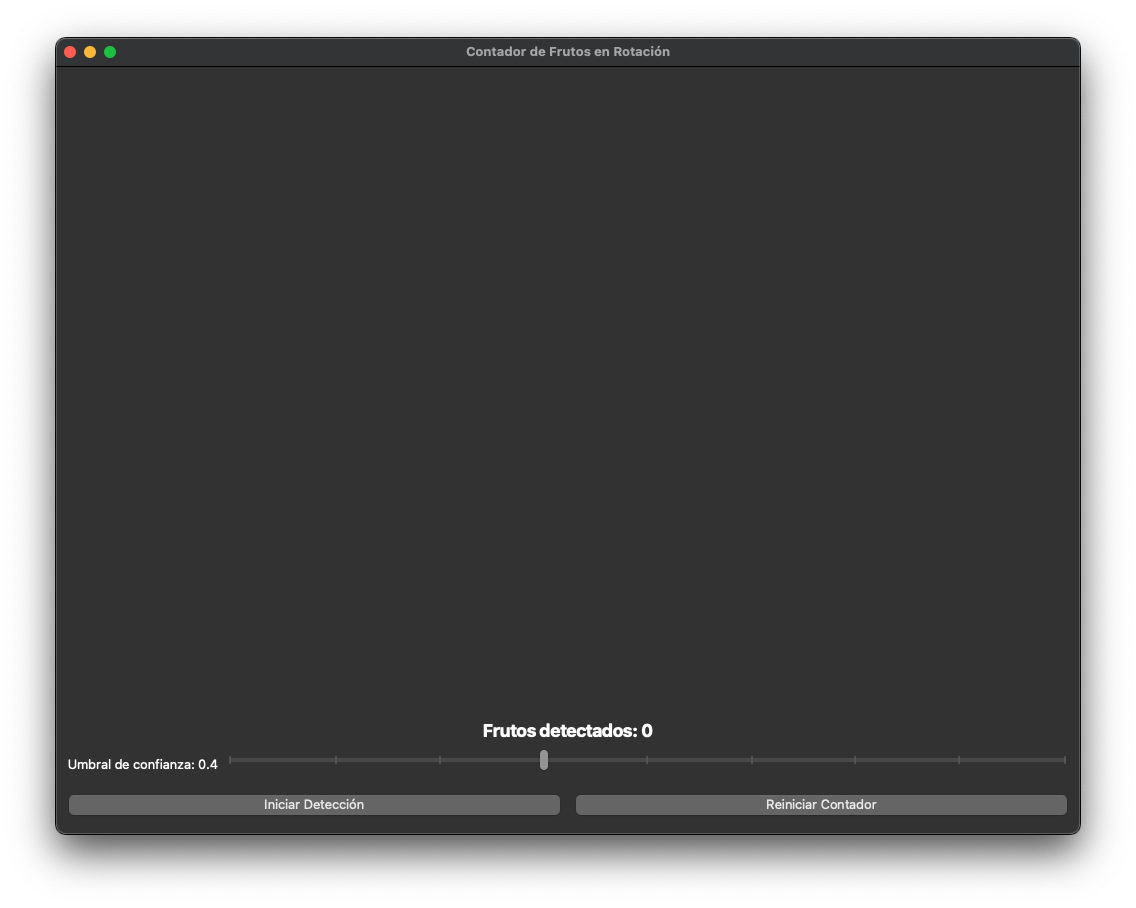
\includegraphics[width=\columnwidth]{images/UI.png}
    \caption{Interfaz gráfica.}
    \label{fig:interfaz}
\end{figure}

% UI-ejecutando.png
\begin{figure}[ht]
    \centering
    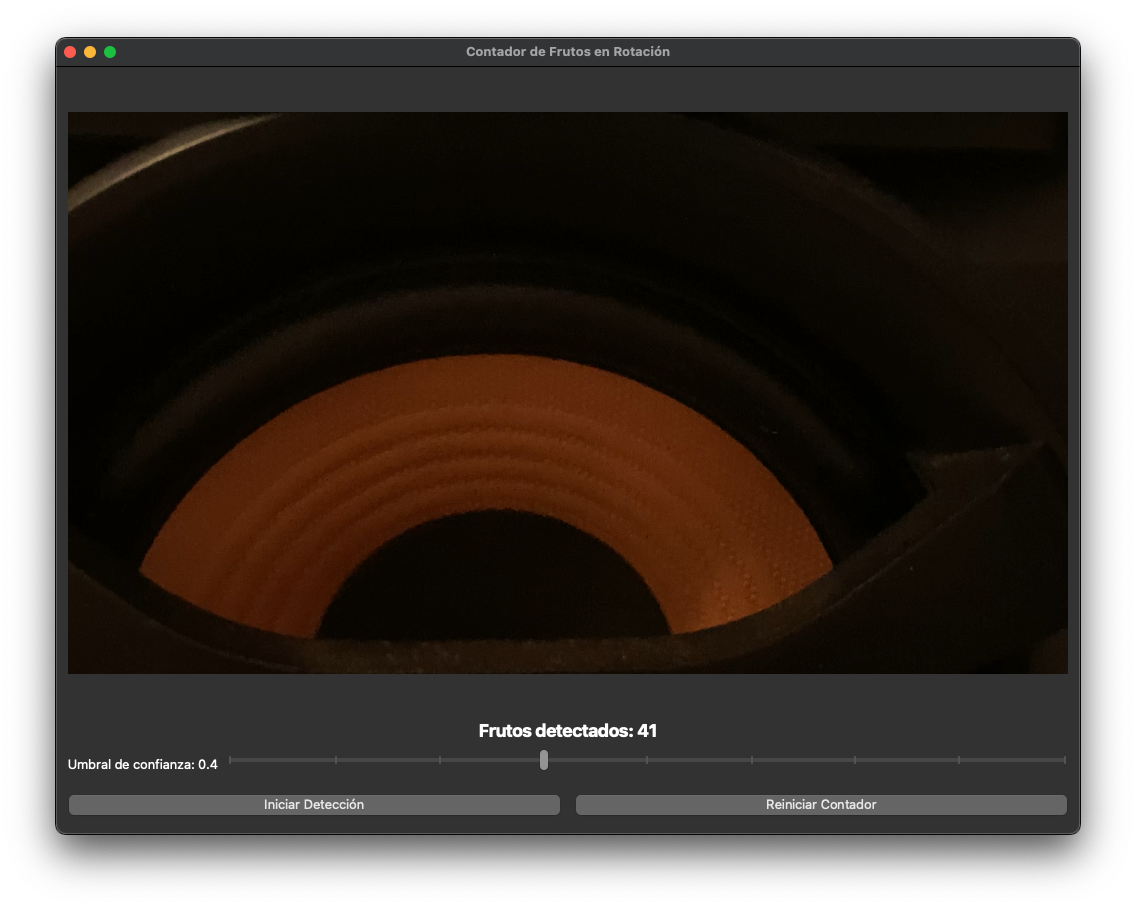
\includegraphics[width=\columnwidth]{images/UI-ejecutando.png}
    \caption{Interfaz gráfica ejecutando la detección de frutos en tiempo real.}
    \label{fig:interfaz-ejecutando}
\end{figure}

% detection.png
\begin{figure}[ht]
    \centering
    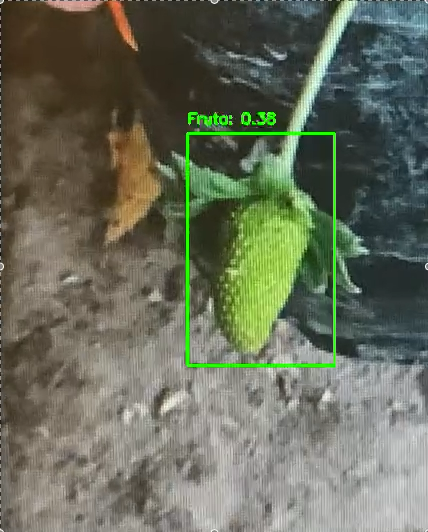
\includegraphics[width=\columnwidth]{images/detection.png}
    \caption{Imagen ejemplificando la detección de frutos en tiempo real.}
    \label{fig:detection}
\end{figure}

% detection2.png
\begin{figure}[ht]
    \centering
    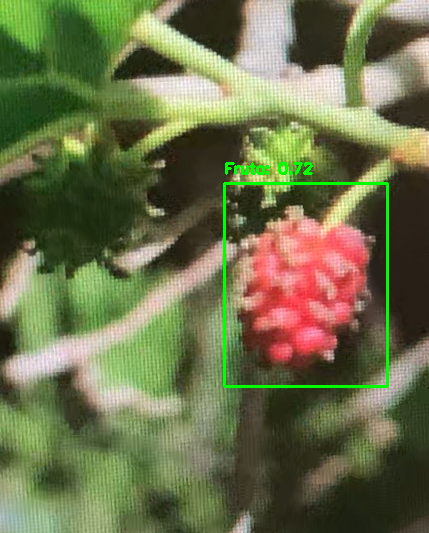
\includegraphics[width=\columnwidth]{images/detection2.png}
    \caption{Imagen ejemplificando la detección de frutos en tiempo real.}
    \label{fig:detection2}
\end{figure}

% detection3.png
\begin{figure}[ht]
    \centering
    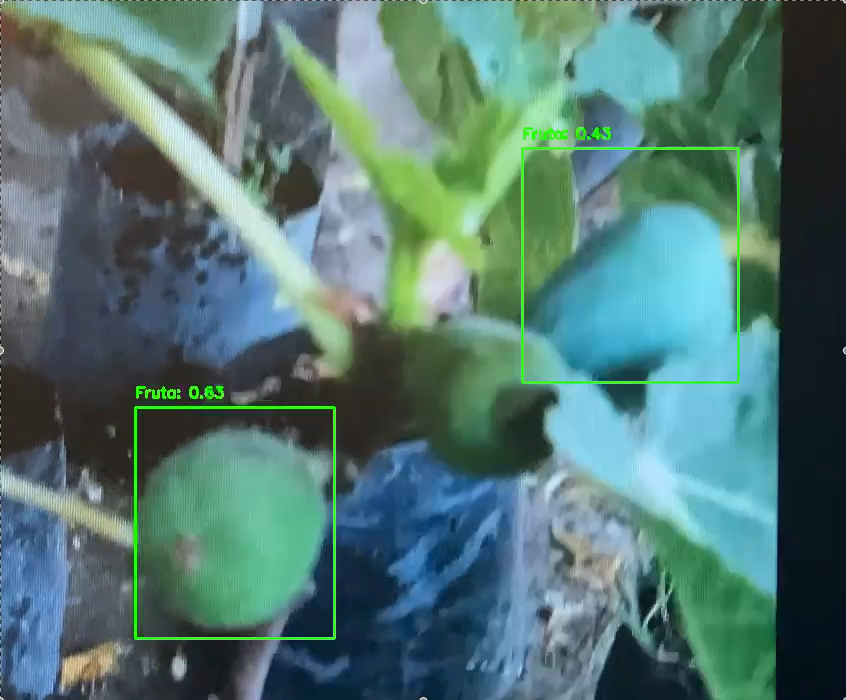
\includegraphics[width=\columnwidth]{images/detection3.png}
    \caption{Imagen ejemplificando la detección de frutos en tiempo real.}
    \label{fig:detection3}
\end{figure}

% detection4.png
\begin{figure}[ht]
    \centering
    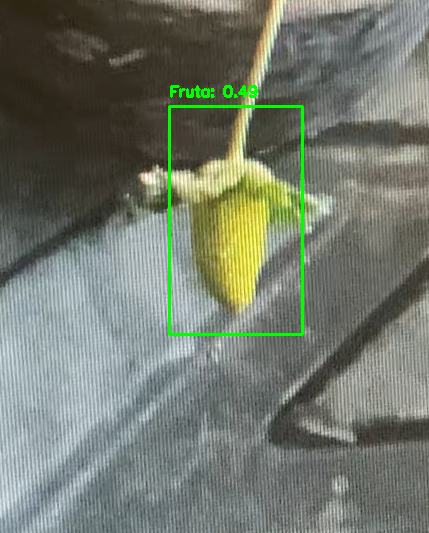
\includegraphics[width=\columnwidth]{images/detection4.png}
    \caption{Imagen ejemplificando la detección de frutos en tiempo real.}
    \label{fig:detection4}
\end{figure}

% real-dec1.png
\begin{figure}[ht]
    \centering
    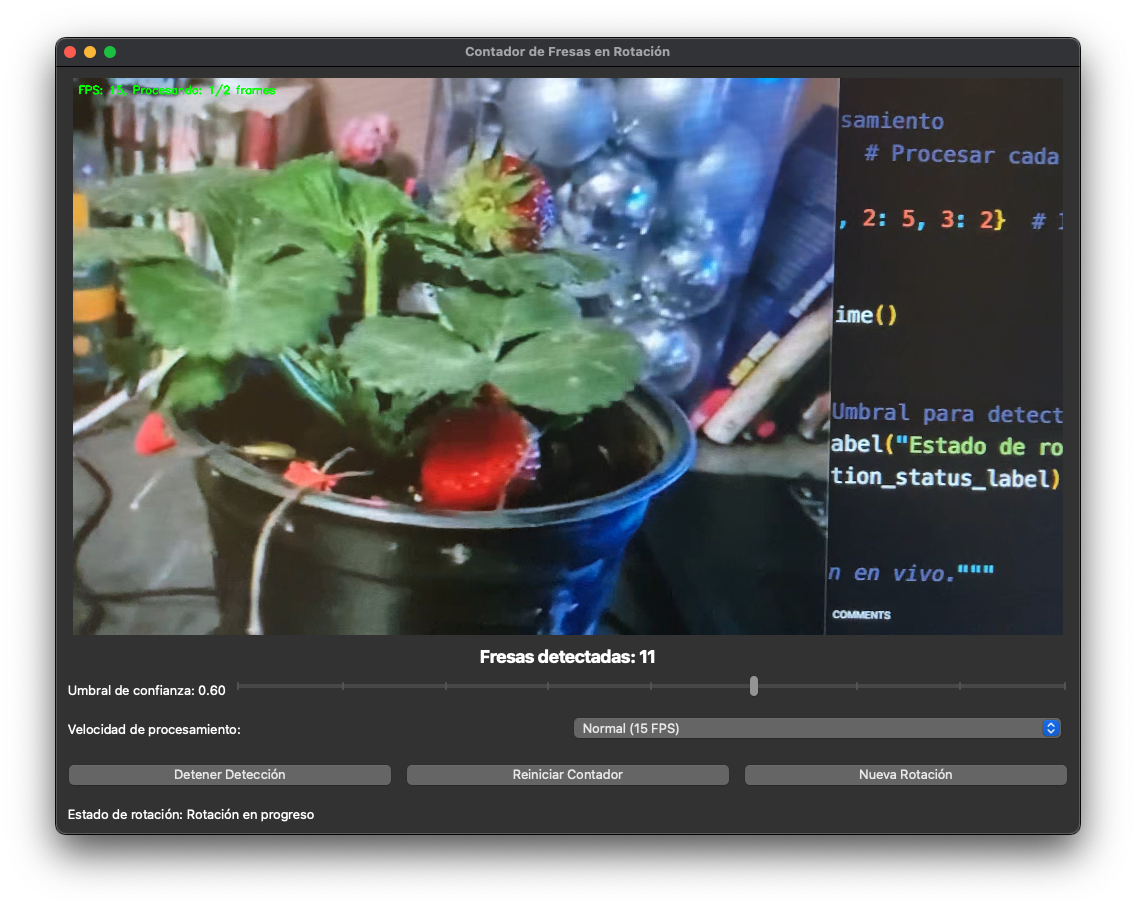
\includegraphics[width=\columnwidth]{images/real-dec1.png}
    \caption{Imagen ejemplificando la detección de frutos en tiempo real en una planta de fresa.}
    \label{fig:real-dec1}
\end{figure}

% real-dec2.png
\begin{figure}[ht]
    \centering
    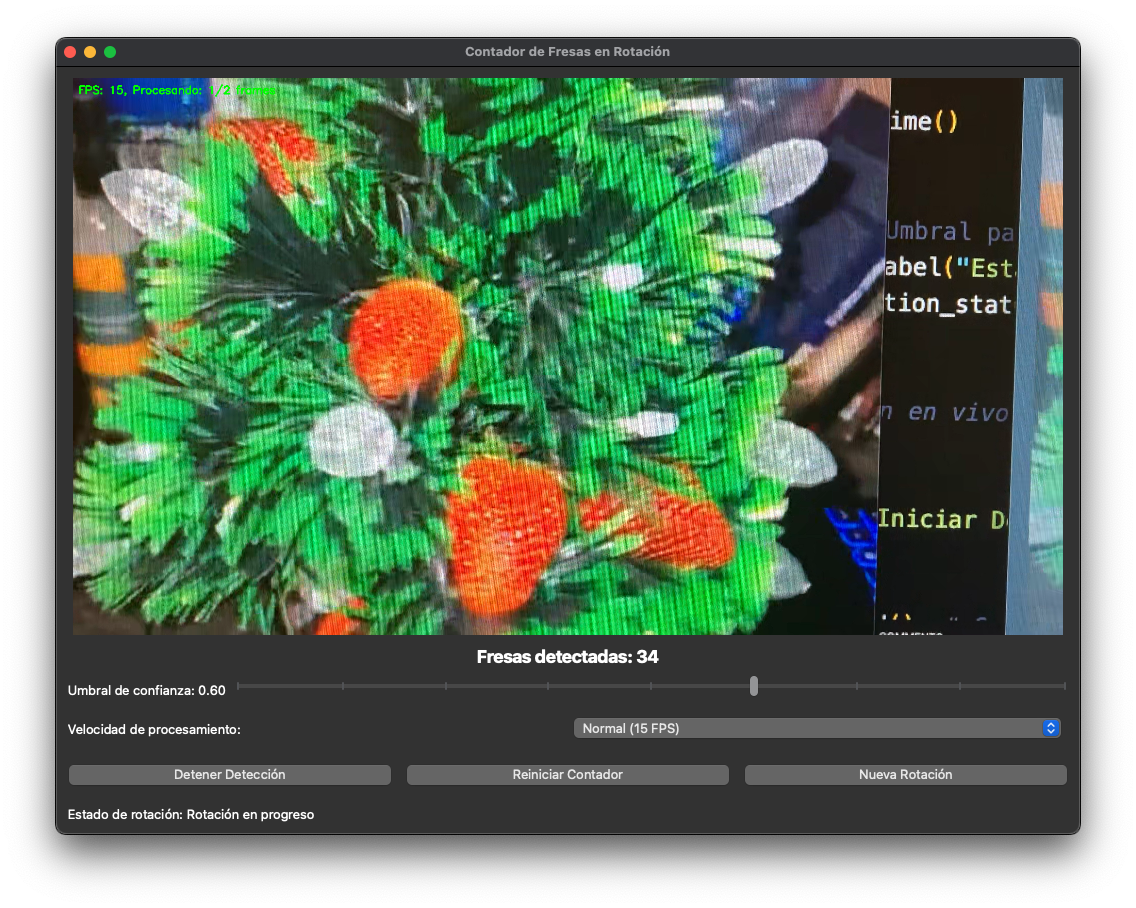
\includegraphics[width=\columnwidth]{images/real-dec2.png}
    \caption{Imagen ejemplificando la detección de frutos en tiempo real en una planta de fresa.}
    \label{fig:real-dec2}
\end{figure}

% P_curve.png
\begin{figure}[ht]
    \centering
    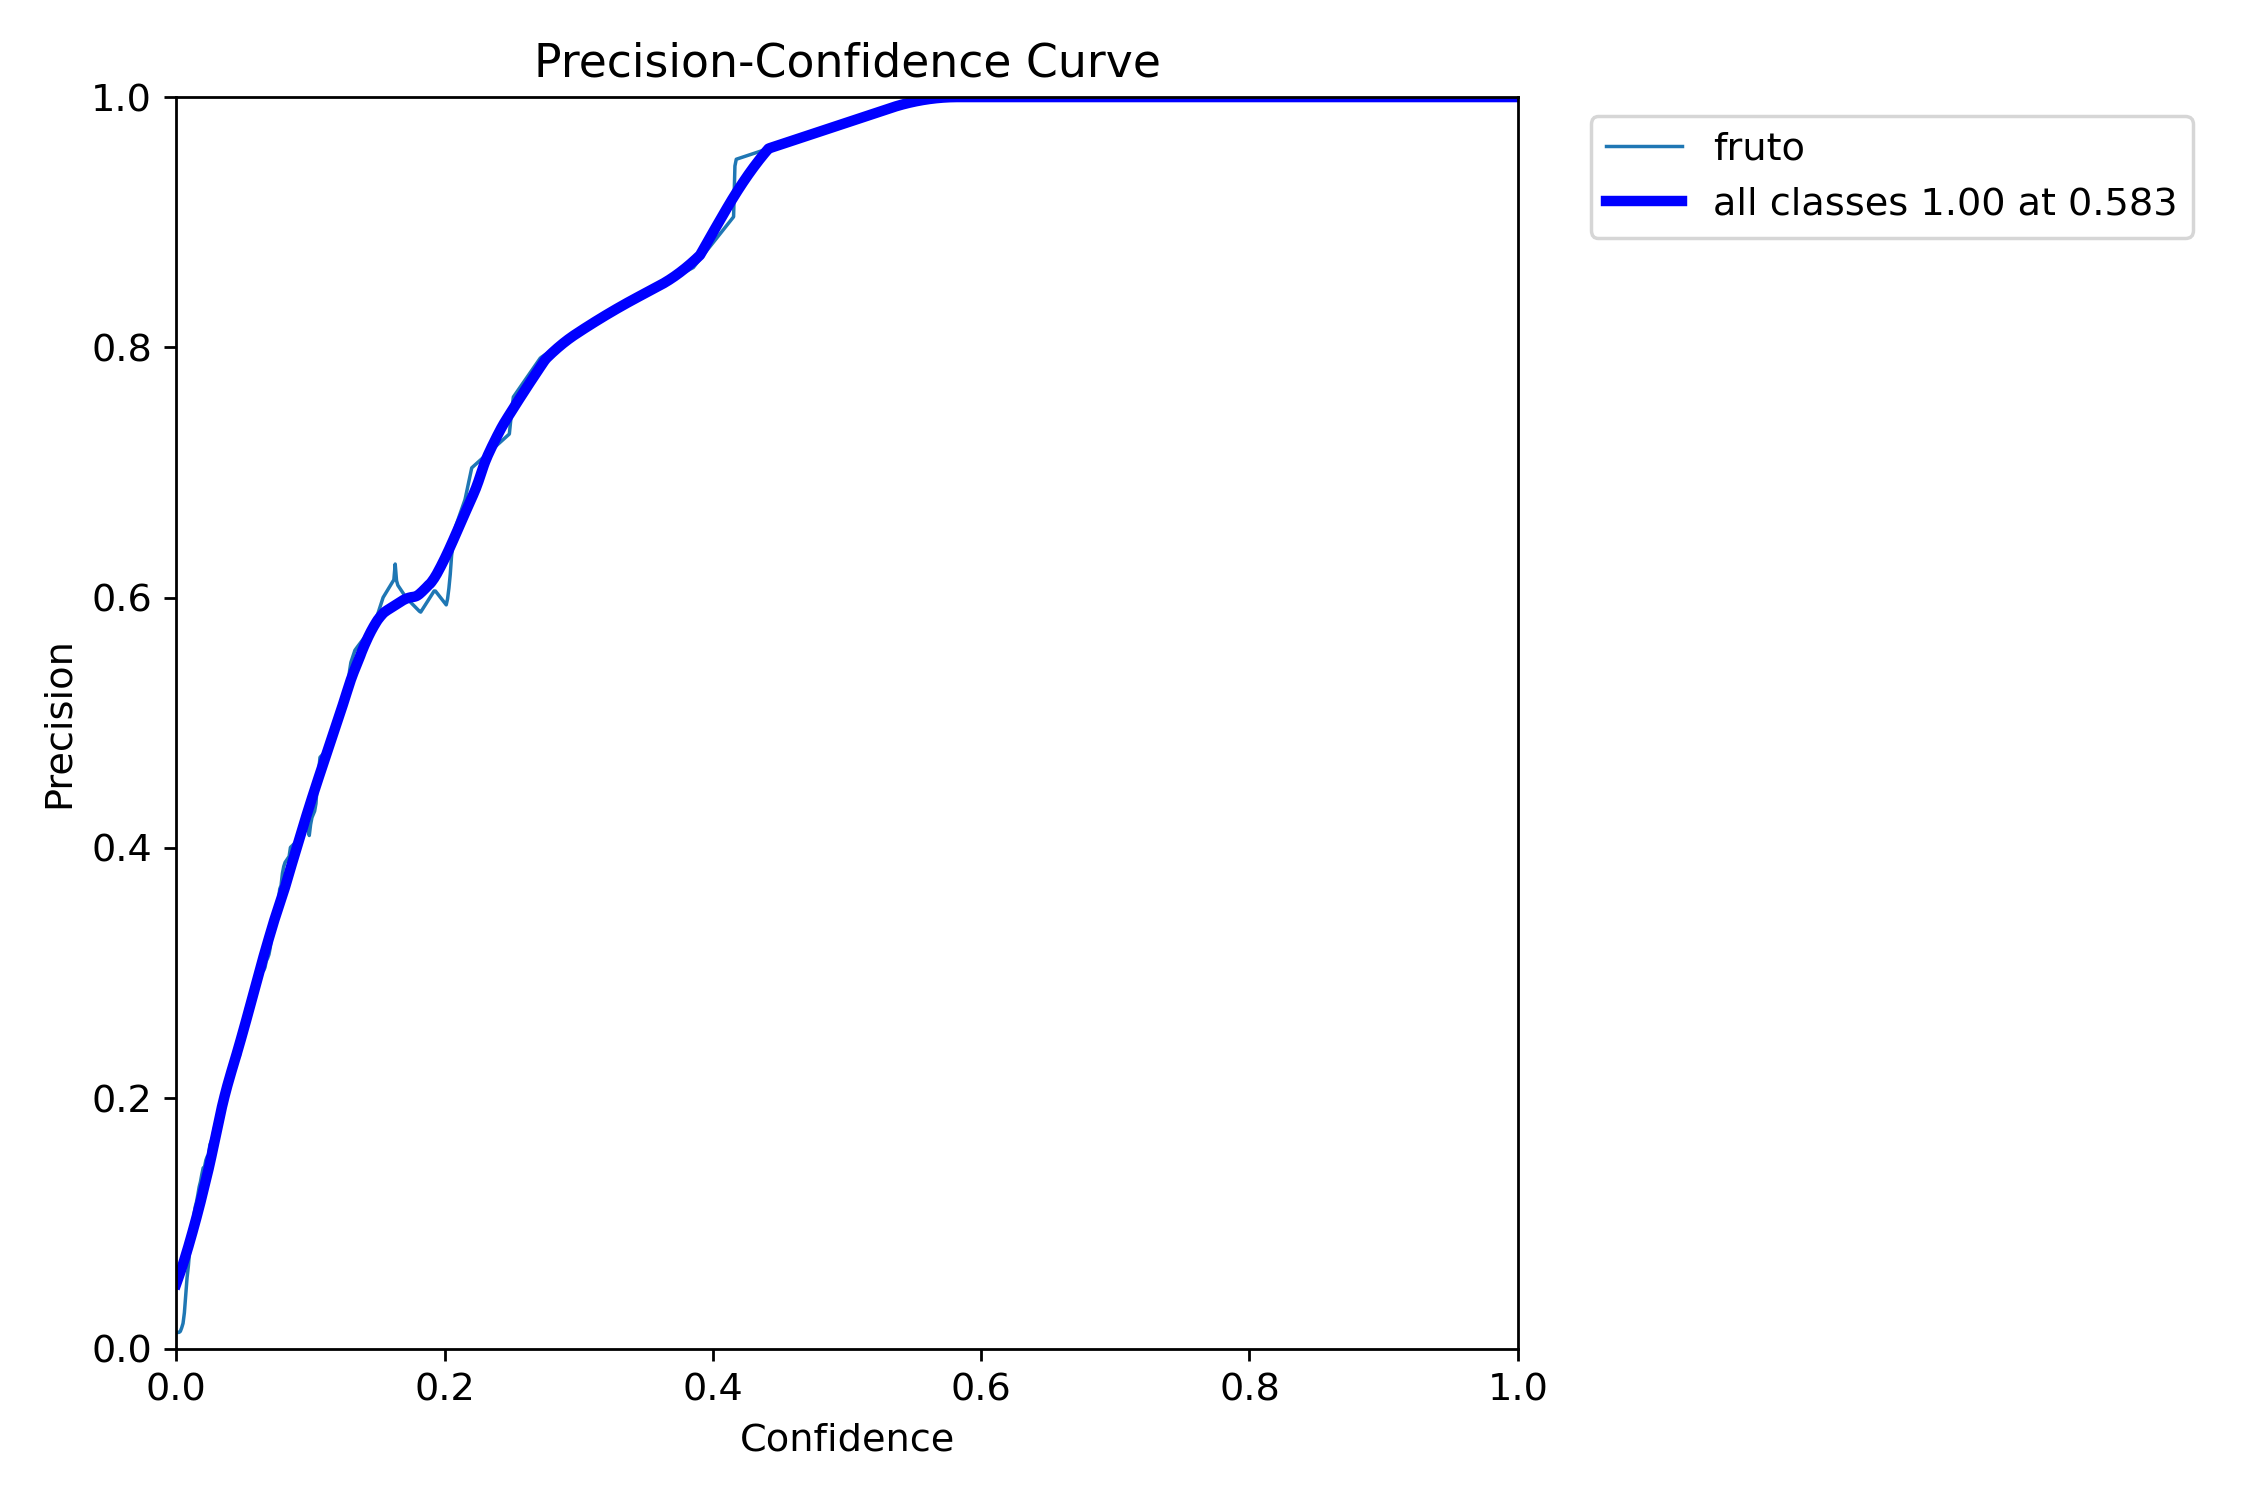
\includegraphics[width=\columnwidth]{images/P_curve.png}
    \caption{Curva de Presición.}
    \label{fig:P_curve}
\end{figure}

% R_curve.png
\begin{figure}[ht]
    \centering
    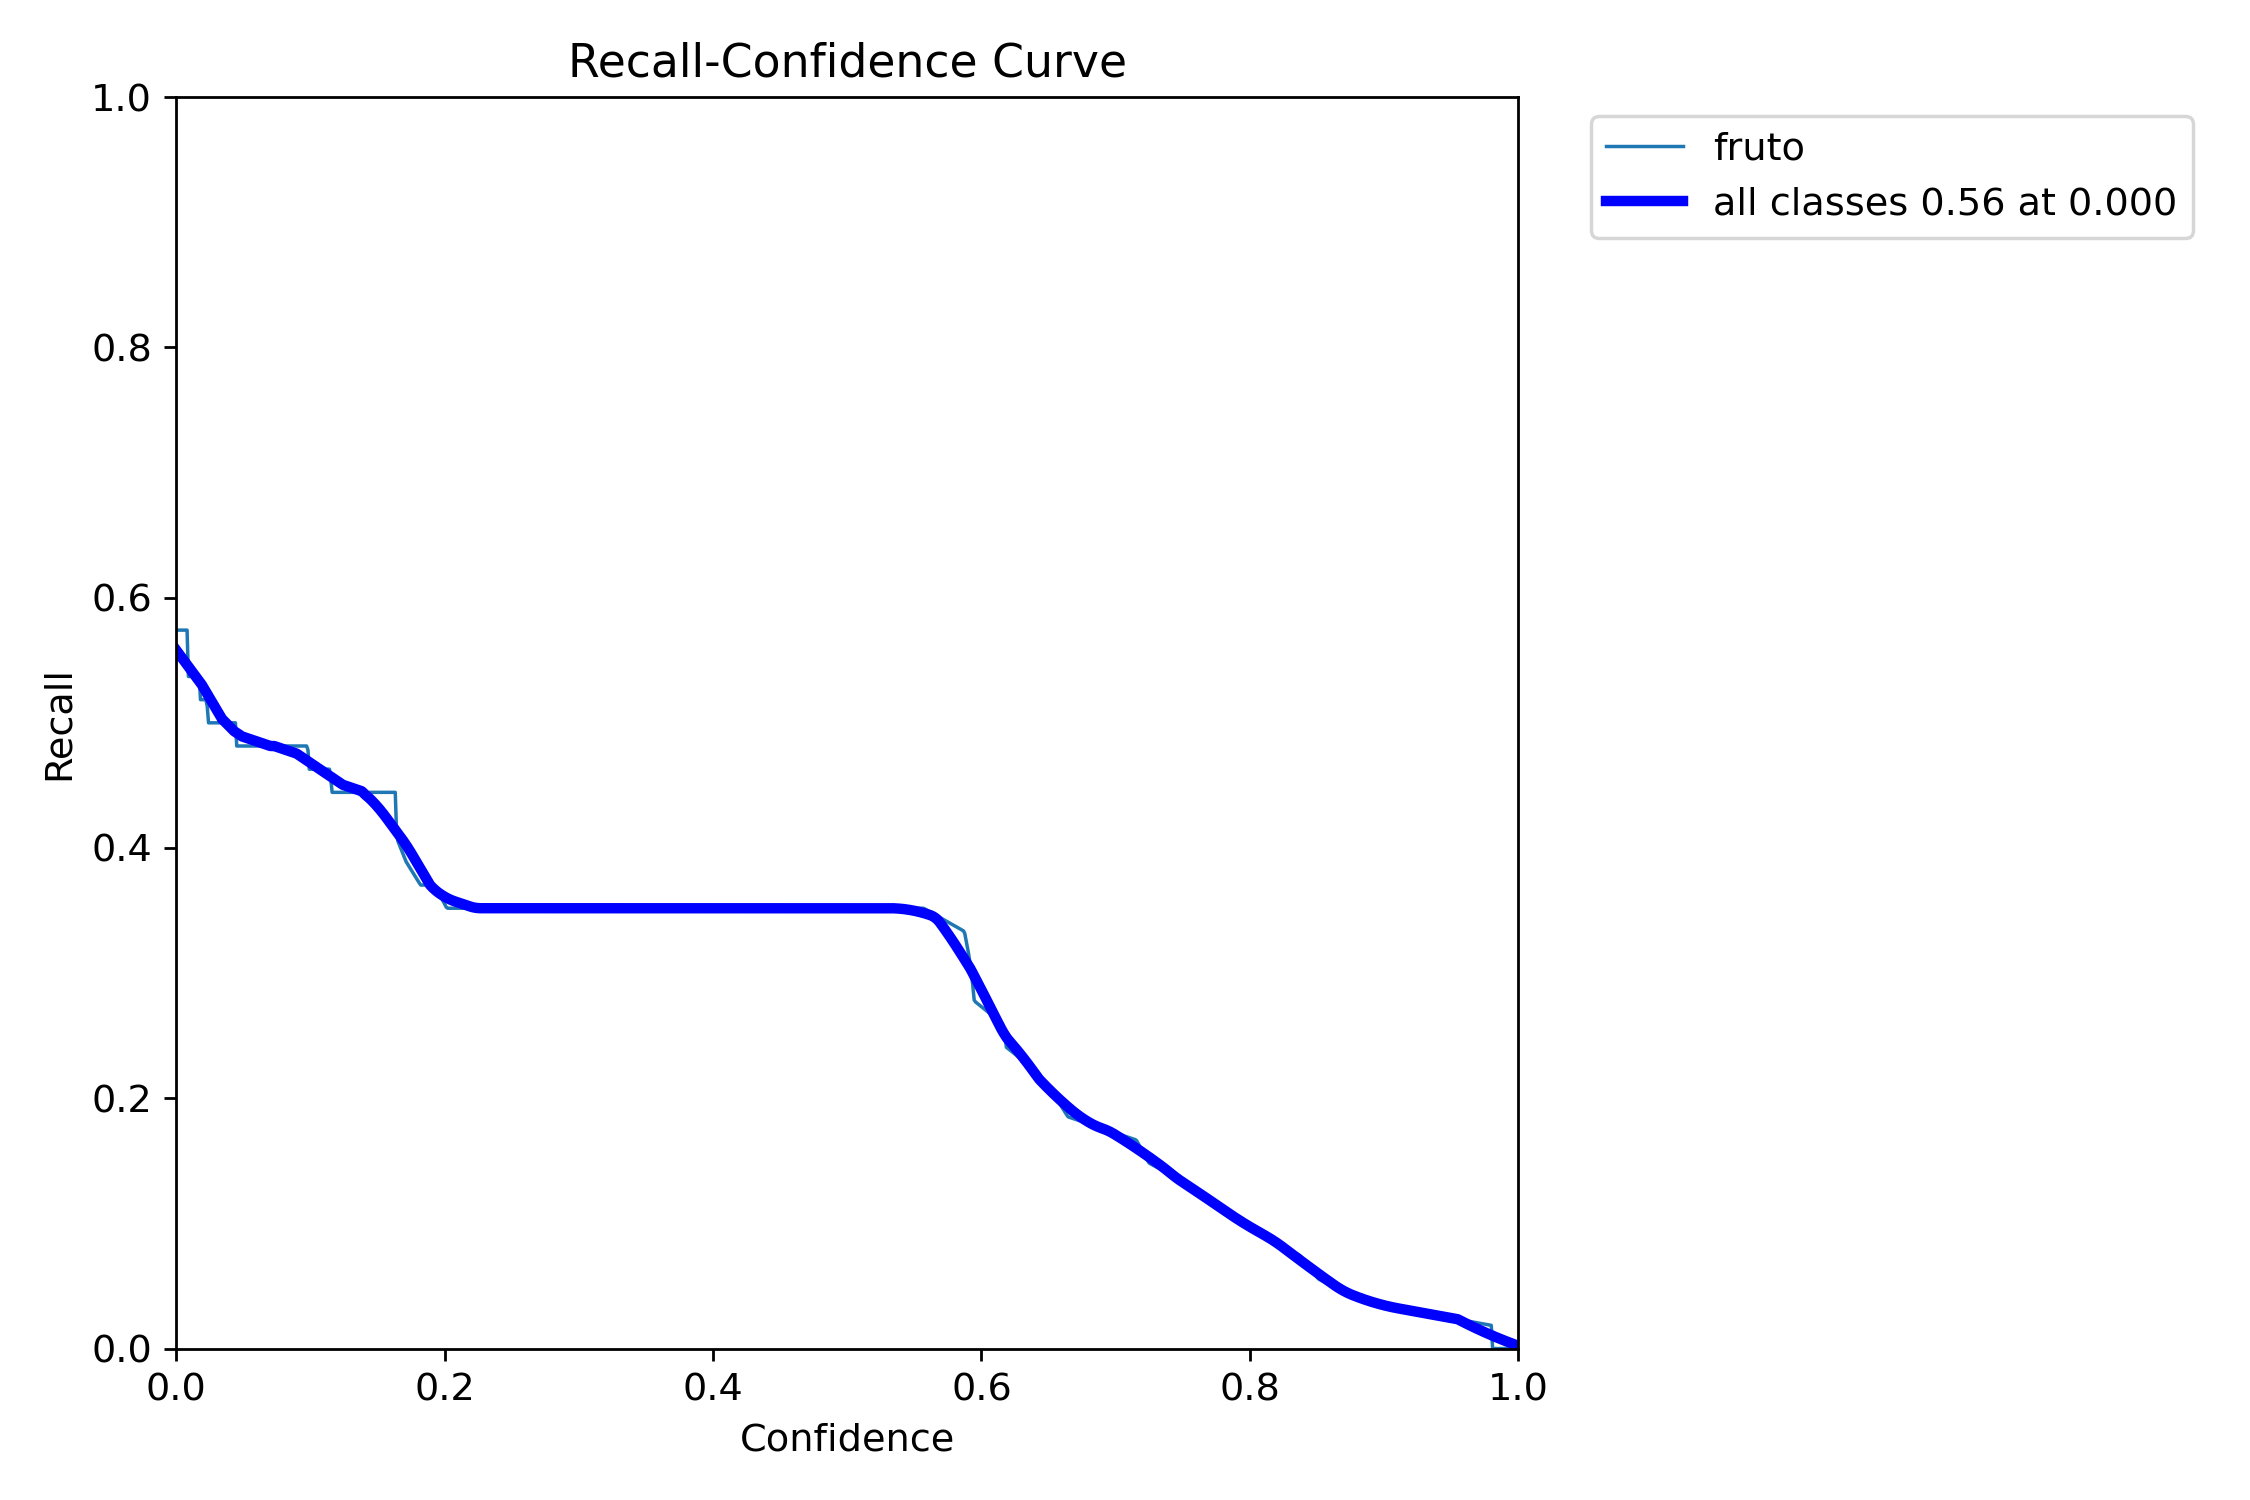
\includegraphics[width=\columnwidth]{images/R_curve.png}
    \caption{Curva de Recall.}
    \label{fig:R_curve}
\end{figure}

% PR_curve.png
\begin{figure}[ht]
    \centering
    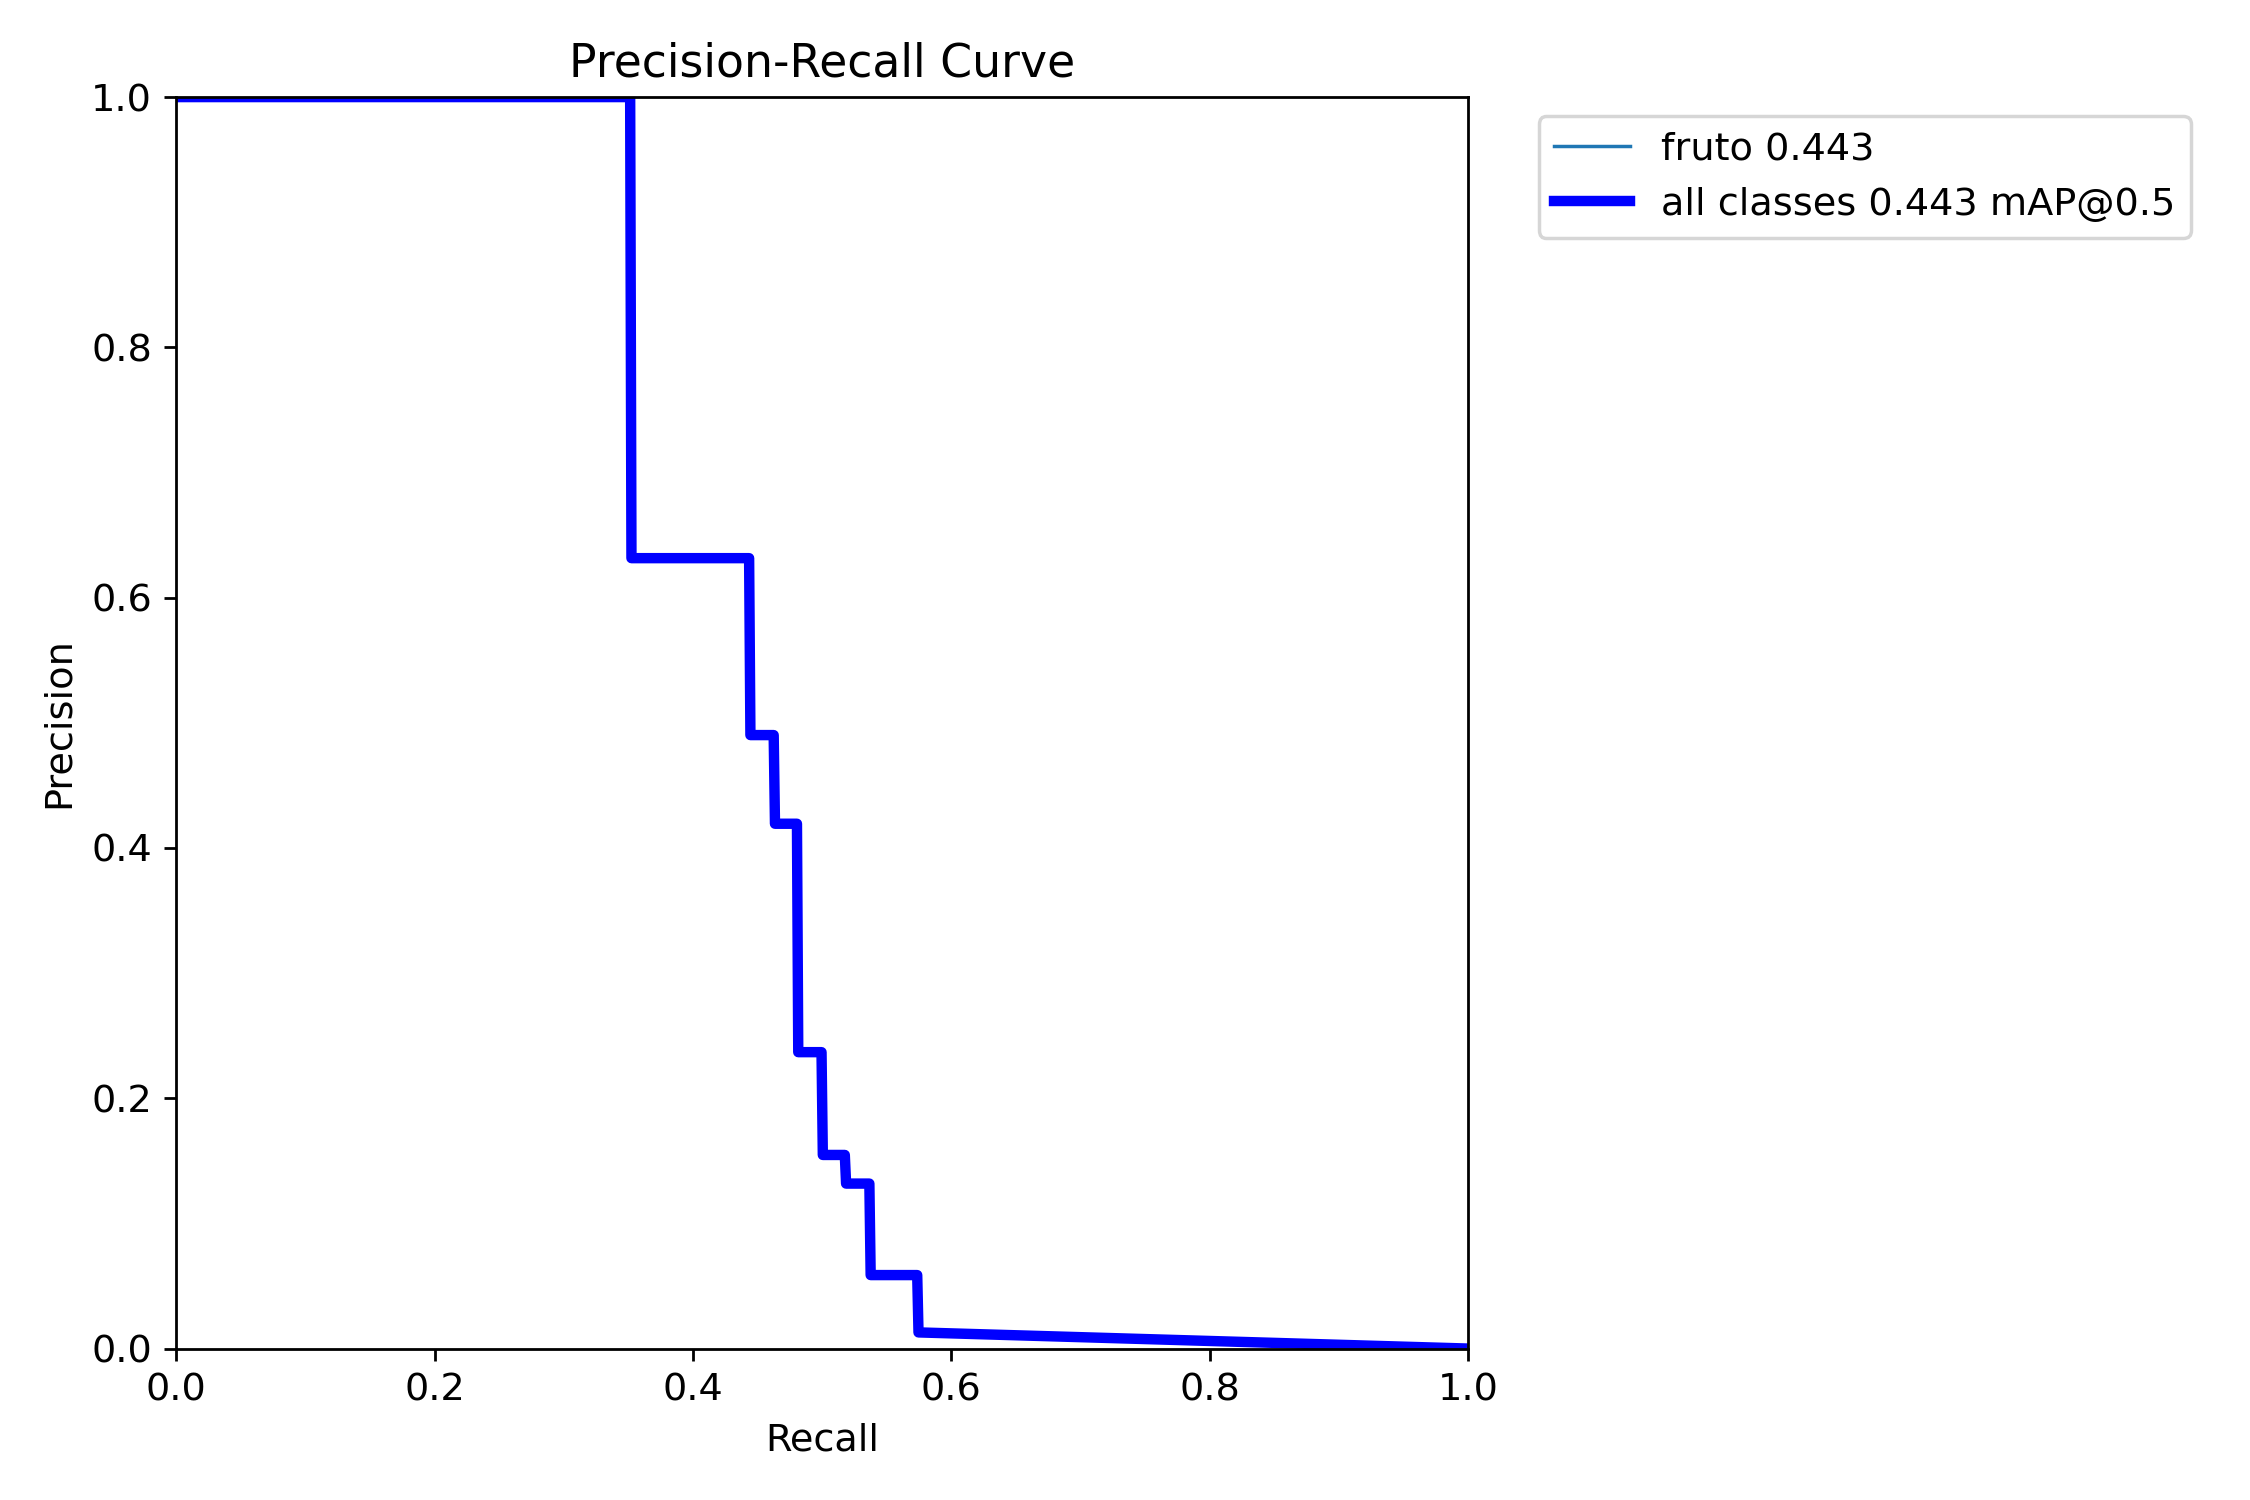
\includegraphics[width=\columnwidth]{images/PR_curve.png}
    \caption{Curva de Presición y Recall.}
    \label{fig:PR_curve}
\end{figure}


%%%%%%%%%%%%%%%%%%%%%%%%%%%%%%%%%%%%%%%%%%%%%%%%%%%%%%%%%%%%%%%%%%%%%%%
\section{Conclusión}
En este trabajo se propuso una solucion al problema de conteo de frutos en tiempo real, utilizando una plataforma giratoria. Se logro implementar un modelo de detección de objetos en tiempo real, que es capaz de detectar frutos en movimiento, sin embargo, el modelo presenta limitaciones en la detección de frutos de colores menos llamativos y en la detección de frutos en posiciones e iluminaciones peculiares, como lo son el fondo de una imagen.


%%%%%%%%%%%%%%%%%%%%%%%%%%%%%%%%%%%%%%%%%%%%%%%%%%%%%%%%%%%%%%%%%%%%%%%
\nocite{calcularRangos}
\addcontentsline{toc}{section}{Referencias} 
\printbibliography
%\balance

\end{document}